\documentclass[../main.tex]{subfiles}

\begin{document}
\قسمت{درباره جنگ ستارگان}

\زیرقسمت{مقدمه}
همانطور که در طول درس هم متوجه شده‌اید، پرهام مجموعه فیلم‌های جنگ ستارگان\پانویس{The Star Wars} را دوست دارد.
در این آزمون قصد داریم یک وب‌سایت ساده برای جمع‌آوری اطلاعات این مجموعه فیلم طراحی کنیم.

\زیرقسمت{وب‌گاه}
وب‌گاهی که پیاده‌سازی می‌کنید، از شمای زیر پیروی می‌کند. در این شِما یک عکس پس‌زمینه وجود داشته و محتوا در قالب یک مستطیل با پس‌زمینه شفاف روی آن نمایش داده می‌شود.
در نظر داشته باشید که عکس پس‌زمینه می‌بایست تمام صفحه را پوشانده باشد و در صورتی که از صفحه بزرگتر باشد \متن‌سیاه{نباید} باعث ایجاد \متن‌لاتین{scrollbar} گردد.
برای اینکه پوشش صفحه کافی باشد از عکس‌هایی با وضوح بالا (مثلا $1920 \corss 1028$) استفاده کنید.
در شرایطی که ابعاد صفحه نمایش کوچکتر از وضوح عکس باشد، می‌بایست قسمتی از وسط عکس نمایش داده شود.
برای تصویر پس‌زمینه حتما از عکس استفاده کنید، برای مثال می‌توانید از \تارنما{https://unsplash.com/s/photos/starwars}{اینجا} استفاده کنید.

\شروع{شکل}[h]
  \تنظیم‌ازوسط
  \درج‌تصویر[scale=0.25]{./swapi-top-level}
  \شرح{طراحی سطح بالا}
\پایان{شکل}

مستطیل میانی تمامی محتویات قابل نمایش شما را می‌بایست شامل شود. این مستطیل می‌بایست تنها به اندازه محتویات باشد اما
برای نمایش زیباتر برای آن \متن‌لاتین{padding} در نظر بگیرید.

\زیرزیرقسمت{محتویات}

آنچه می‌بایست نمایش دهید اطلاعات فیلم‌های ۱ تا ۶ جنگ ستارگان از تارنمای زیر است:

\begin{latin}
  \url{https://swapi.dev/}
\end{latin}

توجه داشته باشید ترتیب نمایش می‌بایست به شرح زیر باشد:

\begin{latin}
  \url{https://swapi.dev/api/films/4}
  \url{https://swapi.dev/api/films/5}
  \url{https://swapi.dev/api/films/6}
  \url{https://swapi.dev/api/films/1}
  \url{https://swapi.dev/api/films/2}
  \url{https://swapi.dev/api/films/3}
\end{latin}

برای هر یک از این فیلم‌ها اطلاعات زیر می‌بایست نمایش داده شود:

\begin{itemize}\begin{latinitems}
  \item title
  \item episode_id
  \item release_date
\end{latinitems}\end{itemize}

و ساختار اطلاعات این فیلم‌ها نیز به شرح زیر است:

\begin{latin}
\begin{minted}[bgcolor=LightGray]{json}
{
  "title": "Revenge of the Sith",
  "episode_id": 3,
  "opening_crawl": "War! The Republic is crumbling\r\nunder attacks by the ruthless\r\nSith Lord, Count Dooku.\r\nThere are heroes on both sides.\r\nEvil is everywhere.\r\n\r\nIn a stunning move, the\r\nfiendish droid leader, General\r\nGrievous, has swept into the\r\nRepublic capital and kidnapped\r\nChancellor Palpatine, leader of\r\nthe Galactic Senate.\r\n\r\nAs the Separatist Droid Army\r\nattempts to flee the besieged\r\ncapital with their valuable\r\nhostage, two Jedi Knights lead a\r\ndesperate mission to rescue the\r\ncaptive Chancellor....",
  "director": "George Lucas",
  "producer": "Rick McCallum",
  "release_date": "2005-05-19",
  "characters": [ ... ],
  "planets": [ ... ],
  "starships": [
    "https://swapi.dev/api/starships/2/",
    ...,
  ],
  "vehicles": [ ... ],
  "species": [ ... ],
  "created": "2014-12-20T18:49:38.403000Z",
  "edited": "2014-12-20T20:47:52.073000Z",
  "url": "https://swapi.dev/api/films/6/"
}
\end{minted}
\end{latin}

همانطور که ساختار اطلاعات نمونه نیز مشخص است برای هر فیلم لیستی از کشتی‌های فضایی استفاده شده در آن قسمت وجود دارد.
برای هر فیلم دکمه‌ای با نام \متن‌لاتین{Starship} وجود دارد که با استفاده از آن اطلاعات کشتی‌های فضایی آن قسمت نمایش داده می‌شود.
برای پیاده‌سازی این قسمت جدید می‌بایست لیست فیلم‌ها حذف شود.
شما می‌بایست برای هر یک از این کشتی‌های فضایی به لینکی که داده شده است تقاضا داده و \متن‌ایتالیک{نام} آن را استخراج کرده
و در این قسمت جدید نمایش دهید.

\شروع{شکل}[h]
  \centering
  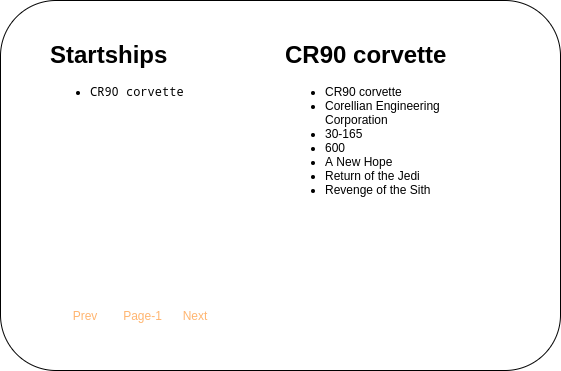
\includegraphics[scale=0.25]{./swapi-content}
  \caption{طراحی مستطیل محتوا}
\پایان{شکل}

کاربر می‌تواند از لیست این کشتی‌فضایی‌ها یکی را انتخاب کرده و جزئیات آن را ببیند.
اگر بخواهیم دقیقتر صحبت کنیم لیست شامل \متن‌ایتالیک{نام} ۱۰ کشتی‌فضایی است
که با کلیک بر روی هر یک اطلاعات جزئی آن شامل \متن‌اتالیک{مدل}، \متن‌ایتالیک{سازنده}، \متن‌ایتالیک{خدمه} و \متن‌ایتالیک{تعداد مسافران} نمایان می‌گردد.
برای نمونه داده‌ای که شما برای یک کشتی فضایی دریافت می‌کنید در ادامه آورده شده است.
در این قسمت هم اطلاعات قبلی حذف شده و اطلاعات جدید نمایش داده می‌شوند.

\begin{latin}
\begin{minted}[bgcolor=LightGray]{json}
{
    "name": "Imperial shuttle",
    "model": "Lambda-class T-4a shuttle",
    "manufacturer": "Sienar Fleet Systems",
    "cost_in_credits": "240000",
    "length": "20",
    "max_atmosphering_speed": "850",
    "crew": "6",
    "passengers": "20",
    "cargo_capacity": "80000",
    "consumables": "2 months",
    "hyperdrive_rating": "1.0",
    "MGLT": "50",
    "starship_class": "Armed government transport",
    "pilots": [
        "http://swapi.dev/api/people/1/",
        "http://swapi.dev/api/people/13/",
        "http://swapi.dev/api/people/14/"
    ],
    "films": [
        "http://swapi.dev/api/films/2/",
        "http://swapi.dev/api/films/3/"
    ],
    "created": "2014-12-15T13:04:47.235000Z",
    "edited": "2014-12-20T21:23:49.900000Z",
    "url": "http://swapi.dev/api/starships/22/''
}
\end{minted}
\end{latin}

در صورتی که قسمت فیلم‌ها نیز دارای اطلاعات باشد می‌بایست نام فیلم‌ها ذکر شود.
دقت کنید برای این امر نیاز به یک تقاضای جداگانه برای فیلم دارید. ساختار \متن‌لاتین{URL}ها در اینجا بسیار ساده می‌باشند ولی در جهت تاکید در قسمت زیر آن‌ها را مرور کرده‌ایم:

\begin{itemize}\begin{latinitems}
  \item https://swapi.dev/api/starships/<id>
  \item https://swapi.dev/api/films/<id>
\end{latinitems}\end{itemize}

در نظر داشته باشید در همه قسمت‌ها نیاز به دکمه بازگشت داریم.

\زیرقسمت{صفحه‌گذاری}

فرض کنید لیست بلندی از آیتم‌ها در اختیار شما قرار گرفته است، در صفحه‌گذاری این لیست را به صفحاتی می‌شکانید که در هر صفحه تعداد مشخصی از اطلاعات وجود دارند. کاربران به جای کارکردن با لیست بلندی از آیتم‌ها با صفحاتی مواجه هستند که تعداد مشخصی از آیتم‌ها را در بر گرفته‌اند. کاربر می‌تواند از قبل در رابطه با تعداد کل صفحات اطلاع داشته باشد و می‌تواند چنین اطلاعی نیز به او داده نشود. همانطور که ادامه هم بیان می‌شود چگونگی پیاده‌سازی این موضوع به خود شما وابسته است.
جزئیات پیاده‌سازی این قسمت کاملا برعهده خودتان می‌باشد.
می‌توانید لیست تمام کشتی‌فضایی‌ها را در ابتدا ساخته و در ادامه صفحه‌گذاری را کاملا در سمت کلاینت انجام دهید یا می‌توانید در هر بار تغییر صفحه لیست کشتی‌فضایی‌ها را دریافت کنید.
در نظر داشته باشید که تمامی فرآیند می‌بایست پویا بوده باشد و هیچ چیز به صورتی دستی در کدتان وارد نشده باشد، به طور دقیق‌تر با تغییر تعداد کشتی‌فضایی‌ها می‌بایست همچنان برنامه شما به طور صحیح به فعالیت خود ادامه دهد.

به طور مثال فرض کنید در مجموع ۲۶ کشتی‌فضایی وجود دارند. یک راه برای پیاده‌سازی صفحه‌گذاری به این ترتیب خواهد بود.

\شروع{شمارش}
\فقره گرفتن تمامی اطلاعات کشتی‌فضایی‌های موجود
\فقره نمایش ۱۰ کشتی‌فضایی در هر صفحه، به این ترتیب دو صفحه با ۱۰ کشتی‌فضایی و یک صفحه با ۶ کشتی‌فضایی خواهیم داشت.
\فقره پیاده‌سازی دکمه‌هایی برای جابجایی بین صفحات
\پایان{شمارش}

\زیرقسمت{انتشار}
پیاده‌سازی یک وب‌سایت بدون قرار دادن آن برای همه، کار کاملی نخواهد بود. از این رو در قسمت نحوه انتشار این وبگاه روی \تارنما{https://github.com}{گیت‌هاب} را مرور می‌کنیم.

در گام اول می‌بایست یک مخزن ایجاد کرده و کد خود را در آن قرار دهید. فایل \متن‌لاتین{index.html} با همین نام می‌بایست در ریشه\پانویس{root} مخزن شما قرار داشته باشد.
در فایل \متن‌لاتین{index.html} می‌توانید به صورت نسبی\پانویس{relative} سایر فایل‌ها مانند عکس یا اسکریپت‌ها و \نقاط‌خ را ارجاع دهید.

در گام بعد می‌بایست از نوار بالا به زبانه \متن‌لاتین{settings} رفته و از منوی سمت چپ گزینه \متن‌لاتین{pages} را انتخاب کنید.
در قسمت \متن‌لاتین{pages} گزینه \متن‌لاتین{None} را انتخاب کرده و آن را به نام شاخه\پانویس{branch} خود تغییر دهید.

\begin{figure}[h]
  \centering
  \includegraphics[scale=0.3]{./github-step-1}
  \caption{زبانه \متن‌لاتین{settings}}
\end{figure}

\begin{figure}[h]
  \centering
  \includegraphics[scale=0.3]{./github-step-2}
  \caption{قسمت \متن‌لاتین{pages} در زبانه \متن‌لاتین{settings}}
\end{figure}

بعد از این وب‌سایت شما از آدرس زیر قابل رویت خواهد بود.

\begin{latin}\begin{center}
https://<username>.github.io/<repo>
\end{center}\end{latin}

که در آن \متن‌لاتین{username} نام کاربری شما در گیت‌هاب و \متن‌لاتین{repo} نام مخزن شماست. این آدرس در قابل یک فایل متنی در کنار سایر موارد پروژه خود بارگذاری نمایید.

\زیرقسمت{نکات پیاده‌سازی}

\شروع{فقرات}
\فقره آنچه در شما آورده شده است برای فهم بهتر شما می‌باشد بنابراین سعی کنید تا حد امکان وب‌سایت را گویا طراحی کنید.
\فقره برای کدهایتان از کامنت استفاده کنید. توضیح کارکرد بلاک‌های \متن‌لاتین{css} اجباری می‌باشد. توابعی و قطعات کد جاوا اسکریپت نیز می‌بایست حداقل یک خط کامنت داشته باشند.
\فقره کامنت فارسی یا انگلیسی موردی ندارد اما از فینگلیش (!) نوشتن پرهیز کنید.
\فقره استفاده از کتابخانه‌ها و فریم‌ورک‌ها در پروژه مجاز \متن‌سیاه{نمی‌باشد}.
\فقره از آنجایی که این پروژه در قالب \متن‌سیاه{امتحان میانترم} می‌باشد از تغییر دادن صورت مساله یا انجام موارد خارج از موارد مطرح شده خودداری کنید.
\پایان{فقرات}

\زیرقسمت{پرسش‌های متداول}

\شروع{توضیحات}
\فقره[پرسش] منظورتان از این که ``درصورتی که ابعاد صفحه مناسب نباشد عکس در وسط زوم شود چیست؟''
مگر قرار نیست عکس ما کل صفحه رو بپوشاند و متناسب با تغییرات صفحه اندازه‌اش نیز تغییر کند؟
\فقره[پاسخ] ببینید عکسی که انتخاب می‌کنید قاعدتا یک اندازه مشخصی دارد که اگر در صفحه جا نشود به اجبار می‌بایست
قسمتی از آن را نمایش دهید، منظور من این بود که این قسمت از وسط عکس بریده شده باشد.

\فقره[پرسش] برای اطلاعاتی که داخل مستطیل میانی قابل نمایش است،
ابتدا باید همه سفینه‌ها در سمت چپ صفحه مشخص باشند، سمت راست اطلاعات هر سفینه انتخابی باشد؟ یا فرمتی که این ها میتونن قرار بگیرند خیلی مهم نیست؟
\فقره[پاسخ] فرمت کلی به این شکل است اما هر تغییری در این قسمت ممکن است.

\فقره[پرسش] هندل کردن \متن‌لاتین{404 Not Found}های \متن‌لاتین{api} چطوری باید باشد؟
\فقره[پاسخ] در حالت اجباری شما با چنین چیزی برخود نمی‌کنید چرا که همیشه از لینک‌های معتبر استفاده کرده
و شناسه فیلم‌ها نیز در کد نوشته شده است.

\فقره[پرسش] کدهای \متن‌لاتین{js} و \متن‌لاتین{html} در چه حد کامنت لازم دارند؟ اگر اسم متغیرها و متدها گویا باشند باز هم لازم است؟
\فقره[پاسخ] در رابطه با \متن‌لاتین{html} تنها نیاز است که قسمت‌های کلی را معرفی کنید،
به طور مثال مشخص کنید از این بخش برای لیست کردن کشتی‌فضایی‌ها استفاده خواهید کرد.
در رابطه \متن‌لاتین{js} در صورتی که از نام‌های مناسب برای توابع و متغیرهای استفاده کنید کفایت خواهد کرد.
در رابطه با \متن‌لاتین{css} همانطور که بیان شد توضیح بلاک‌ها اجباری می‌باشد.
به طور مثال این بلاک قصد دارد عکس پس زمینه با که با \متن‌لاتین{\#background} مشخص شده است را در تمام صحفه نمایش داده و در وسط قرار دهد.

\پایان{توضیحات}

\end{document}
